\documentclass{math}

\usepackage{tikz}

\title{Linear Algebra}
\author{Alvin Lin}
\date{August 2017 - December 2017}

\begin{document}

\maketitle

\section*{Linear Algebra}
The study of linear algebra is about two basic things. We study
\textbf{vector spaces} and structure preserving maps between vector
spaces. A \textbf{vector space} is set \( v \) with two binary operations,
addition and scalar multiplcation. A vector space will satisfy various
distributive identities.
\[ \R^2, \R^3, \dots, \R^n \]
are all vector spaces.

\section*{Vectors}
A \textbf{vector} is a directed line segment corresponding to the displacement
from points \( A \) to \( B \) (in \( \R^2 \)). If a vector starts at the
origin, we will say that the vector is in standard position. We can represent
them as row vectors or column vectors depending on convenience. Each is an
ordered pair.
\[ \vec{v} =
  \begin{bmatrix}
    2 & 3 \\
  \end{bmatrix} \]
\[ \vec{v} =
  \begin{bmatrix}
    2 \\
    3
  \end{bmatrix}
\]
The zero vector (\( \vec{0} \)) is a special vector.
\[ \vec{0} =
  \begin{bmatrix}
    0 & 0
  \end{bmatrix}
\]
Let \( \vec{v}\in\R^2 \):
\[ \vec{v}+\vec{0}=\vec{0}+\vec{v}=\vec{v} \]

\subsection*{Adding Vectors in \( \R^2 \)}
Take the following:
\begin{align*}
  \vec{v} &= \langle v_1,v_2\rangle \\
  \vec{w} &= \langle w_1,w_2\rangle \\
  \vec{v}+\vec{w} &= \langle v_1+w_1,v_2+w_2\rangle
\end{align*}
Example:
\begin{align*}
  \vec{v} &= \langle1,2\rangle \\
  \vec{w} &= \langle3,4\rangle \\
  \vec{v}+\vec{w} &= \langle1+3,2+4\rangle = \langle4,6\rangle
\end{align*}

\subsection*{Scalar Multiplication}
Let \( c \) be a scalar and let \( \vec{v} = \langle v_1,v_2\in\R^2 \).
\[ c\cdot\vec{v} = c\langle v_1,v_2\rangle = \langle cv_1,cv_2\rangle \]
Example:
\[ 2\cdot\langle3,4\rangle = \langle2(3),2(4)\rangle = \langle6,8\rangle \]
If \( c>0 \), then \( c\cdot\vec{v} \) points in the same direction as
\( \vec{v} \). \\
If \( c<0 \), then \( c\cdot\vec{v} \) points in the opposite
direction as \( \vec{v} \). \\
If \( |c|>1 \), then \( c\cdot\vec{v} \) is \( \vec{v} \) stretched by a factor
of \( c \). \\
If \( |c|<1 \), then \( c\cdot\vec{v} \) is \( \vec{v} \) compressed by a factor
of \( c \).

\subsection*{Vectors in \( \R^3 \)}
\[ \R^3 = \{(x,y,z)\mid x,y,z\in\R\} \]
Similarly, vectors in \( \R^n \) are:
\[ \R^n = \{(x_1,x_2,\dots,x_n)\mid all\ x_i\in\R\} \]
Let \( \vec{u},\vec{v}\in\R^n \), let \( c\in\R \):
\begin{align*}
  \vec{u}+\vec{v} &= \langle u_1,u_2,\dots,u_n\rangle +
    \langle v_1,v_2,\dots,v_n\rangle +
    \langle u_1+v_1,u_2+v_2,\dots,u_n+v_n\rangle \\
  c\vec{v} &= c\langle v_1,v_2,\dots,v_n\rangle =
    \langle cv_1,cv_2,\dots,cv_n\rangle
\end{align*}

\subsection*{Algebraic Properties of \( \R^n \)}
Let:
\begin{align*}
  \vec{u} &= \langle u_1,u_2,\dots,u_n\rangle\in\R^n \\
  \vec{v} &= \langle v_1,v_2,\dots,v_n\rangle\in\R^n \\
  \vec{w} &= \langle w_1,w_2,\dots,w_n\rangle\in\R^n
\end{align*}
Let \( c,d\in\R \) (scalars):
\begin{enumerate}
  \item Commutative
    \[ \vec{u}+\vec{v} = \vec{v}+\vec{u} \]
  \item Associative
    \[ (\vec{u}+\vec{v})+\vec{w} = \vec{u}+(\vec{v}+\vec{w}) \]
  \item
    \[ \vec{u}+\vec{0} = \vec{0}+\vec{u} = \vec{u} \]
  \item
    \[ \vec{u}+(-\vec{u}) = \vec{0} \]
  \item Distributive
    \[ c(\vec{u}+\vec{v}) = c\vec{u}+c\vec{v} \]
  \item
    \[ (c+d)\vec{u} = c\vec{u}+d\vec{u} \]
  \item
    \[ c(d\vec{u}) = (cd)\vec{u} \]
  \item
    \[ 1\vec{u} = \vec{u} \]
\end{enumerate}
Proof of (1):
\begin{align*}
  \vec{u}+\vec{v} &= \langle u_1,u_2,\dots,u_n\rangle+
    \langle v_1,v_2,\dots,v_n\rangle \\
  &= \langle u_1+v_1,u_2+v_2,\dots,u_n+v_n\rangle \\
  &= \langle v_1+u_1,v_2+u_2,\dots,v_n+u_n\rangle \\
  &= \langle v_1,v_2,\dots,v_n\rangle+
    \langle u_1,u_2,\dots,u_n\rangle \\
  &= \vec{v}+\vec{u}
\end{align*}
Proof of (2):
\begin{align*}
  (\vec{u}+\vec{v})+\vec{w} &= (\langle u_1,\dots,u_n\rangle+
    \langle v_1,\dots,v_n\rangle)+\langle w_1,\dots,w_n\rangle \\
  &= \langle u_1+v_1,\dots,u_n+v_n\rangle+
    \langle w_1,\dots,w_n\rangle \\
  &= \langle(u_1+v_1)+w_1,\dots,(u_n+v_n)+w_n\rangle \\
  &= \langle u_1,\dots,u_n\rangle +
    (\langle v_1+w_1,\dots,v_n+w_n) \\
  &= \vec{u}+(\langle v_1,\dots,v_n\rangle+
    \langle w_1,\dots,w_n\rangle) \\
  &= \vec{u}+(\vec{v}+\vec{w})
\end{align*}
Proof of (3):
\begin{align*}
  \vec{u}+\vec{0} &= \langle u_1,u_2,\dots,u_n\rangle+
    \langle0,0,\dots,0\rangle \\
  &= \langle u_1+0,u_2+0,\dots,u_n+0\rangle \\
  &= \langle u_1,u_2,\dots,u_n\rangle = \vec{u}
\end{align*}
Proof of (4):
\begin{align*}
  \vec{u}+(-\vec{u}) &= \langle u_1,u_2,\dots,u_n\rangle+
    \langle-u_1,-u_2,\dots,-u_n\rangle \\
  &= \langle u_1-u_1,u_2-u_2,\dots,u_n-u_n\rangle \\
  &= \langle0,0,\dots,0\rangle = \vec{0}
\end{align*}
Proof of (5):
\begin{align*}
  c(\vec{u}+\vec{v}) &= c(\langle u_1,u_2,\dots,u_n\rangle+
    \langle v_1,v_2,\dots,v_n\rangle) \\
  &= c(\langle u_1+v_1,u_2+v_2,\dots,u_n+v_n\rangle) \\
  &= \langle c(u_1+v_1),c(u_2+v_2),\dots,c(u_n+v_n)\rangle \\
  &= \langle cu_1+cv_1,cu_2+cv_2,\dots,cu_n+cv_n\rangle \\
  &= \langle cu_1,cu_2,\dots,cu_n\rangle+
    \langle cv_1,cv_2,\dots,cv_n\rangle \\
  &= c\langle u_1,u_2,\dots,u_n\rangle+
    c\langle v_1,v_2,\dots,v_n\rangle \\
  &= c\vec{u}+c\vec{v}
\end{align*}

\subsection*{Linear Combinations}
Let \( \vec{v_1},\vec{v_2},\dots,\vec{v_k}\in\R^n \). We say
\( \vec{v} \) is a \textbf{linear combination} of
\( \vec{v_1},\dots,\vec{v_k} \) if there exists scalars
\( c_1,\dots,c_k \) such that:
\[ \vec{v} = \sum_{i=1}^kc_i\vec{v_i} =
  c_1\vec{v_1}+c_2\vec{v_2}+\dots+c_n\vec{v_n} \]
Example in \( \R^3 \):
Let:
\begin{align*}
  \vec{v} &=
    \begin{bmatrix}
      2 \\ -2 \\ -1
    \end{bmatrix} \quad
  \vec{v_1} =
    \begin{bmatrix}
      1 \\ 0 \\ -1
    \end{bmatrix} \\
  \vec{v_2} &=
    \begin{bmatrix}
      2 \\ -3 \\ 1
    \end{bmatrix} \quad
  \vec{v_3} =
    \begin{bmatrix}
      5 \\ -4 \\ 0
    \end{bmatrix}
\end{align*}
Claim: \( \vec{v} \) is a linear combination of
\( \vec{v_1},\vec{v_2},\vec{v_3} \): \\
We must find \( c_1,c_2,c_3 \) such that:
\[ \vec{v} = c_1\vec{v_1}+c_2\vec{v_2}+c_3\vec{v_3} \]

\subsection*{Dot Product}
Let:
\begin{align*}
  \vec{u} &=
    \begin{bmatrix}
      u_1 \\ u_2 \\ \vdots \\ u_n
    \end{bmatrix} \\
  \vec{v} &=
    \begin{bmatrix}
      v_1 \\ v_2 \\ \vdots \\ v_n
    \end{bmatrix} \\
  \vec{u}\cdot\vec{v} &= \sum_{i=1}^nu_iv_i \\
  &= u_1v_1+u_2v_2+\dots+u_nv_n
\end{align*}

\subsection*{Rules for the Dot Product}
Let \( \vec{u},\vec{v},\vec{w}\in\R^n \), \( c \) is a scalar:
\begin{enumerate}
  \item
    \[ \vec{u}\cdot\vec{v} = \vec{v}\cdot\vec{u} \]
  \item
    \[ \vec{u}\cdot(\vec{v}+\vec{w}) =
      \vec{u}\cdot\vec{v}+\vec{u}\cdot\vec{w} \]
  \item
    \[ (c\vec{u})\cdot\vec{v} = c(\vec{u}\cdot\vec{v}) \]
  \item
    \[ \vec{u}\cdot\vec{u}\geq0 \]
    \[ \vec{u}\cdot\vec{u} = 0\ \textrm{iff}\ \vec{u} = \vec{0} \]
\end{enumerate}
Proof for (1):
\begin{align*}
  \vec{u}\cdot\vec{v} &= \sum_{i=1}^nu_iv_i \\
  &= \sum_{i=1}^nv_iu_i \\
  &= \vec{v}\cdot\vec{u}
\end{align*}
Proof for (2):
\begin{align*}
  \vec{u}\cdot(\vec{v}+\vec{w}) &=
    \vec{u}\cdot(\langle v_1+w_1,\dots,v_n+w_n\rangle) \\
  &= \sum_{i=1}^nu_i(v_i+w_i) \\
  &= \sum_{i=1}^n(u_iv_i+u_iw_i) \\
  &= \sum_{i=1}^nu_iv_i+\sum_{i=1}^nu_iw_i \\
  &= \vec{u}\cdot\vec{v}+\vec{u}\cdot\vec{w}
\end{align*}
Proof for (3):
\begin{align*}
  \sum_{i=1}^n(cu_i)v_i &= \sum_{i=1}^nc(u_iv_i) \\
  &= c\sum_{i=1}^nu_iv_i \\
  &= c(\vec{u}\cdot\vec{v})
\end{align*}
Proof for (4):
\begin{align*}
  \vec{u}\cdot\vec{u} &= \sum_{i=1}^nu_iu_i \\
  &= \sum_{i=1}^n(u_i)^2
\end{align*}
\( (u_1)^2 \) is non-negative, therefore the summation must be greater than
or equal to 0.

\subsection*{Norm or Length of a Vector}
Let:
\begin{align*}
  \vec{v}\in\R^n \quad \vec{v} &= \begin{bmatrix}
    v_1 \\ v_2 \\ \vdots \\ v_N
  \end{bmatrix} \\
  \|\vec{v}\| &= \sqrt{\vec{v}\cdot\vec{v}} \\
  &= \sqrt{\sum_{i=1}^n(v_1)^2}
\end{align*}

\subsubsection*{Example}
In \( \R^2 \), consider \( \vec{v} = \begin{bmatrix}3 \\ 4\end{bmatrix} \).
Calculate \( |\vec{v}| \).
\[ \|\vec{v}\| = \sqrt{3^2+4^2} = \sqrt{9+16} = \sqrt{25} = 5 \]

\subsubsection*{Properties of a vector norm}
\[ |\vec{v}| = 0 \iff \vec{v} = \vec{0} \]
This is true because \( \|\vec{v}\| = 0 \iff \vec{v}\cdot\vec{v} = 0 \iff
  \vec{v} = \vec{0} \).
\[ \|c\vec{v}\| = |c|\|\vec{v}\| \]
Proof:
\begin{align*}
  \|c\vec{v}\|^2 &= (c\vec{v})\cdot(c\vec{v}) \\
  &= c^2(\vec{v}\cdot\vec{v}) \\
  &= c^2\|\vec{v}\|^2 \\
  \sqrt{\|c\vec{v}\|^2} &= \sqrt{c^2\|\vec{v}\|^2} \\
  \|\vec{v}\| = |c|\|\vec{v}\|
\end{align*}

\subsection*{Unit Vectors}
A \textbf{unit vector} is a vector of length 1. In \( \R^2 \):
\begin{align*}
  \vec{e_1} &= \begin{bmatrix}
    1 \\ 0
  \end{bmatrix} \\
  \vec{e_2} &= \begin{bmatrix}
    0 \\ 1
  \end{bmatrix}
\end{align*}
In \( \R^3 \):
\begin{align*}
  \vec{e_1} &= \begin{bmatrix}
    1 \\ 0 \\ 0
  \end{bmatrix} \\
  \vec{e_2} &= \begin{bmatrix}
    0 \\ 1 \\ 0
  \end{bmatrix} \\
  \vec{e_3} &= \begin{bmatrix}
    0 \\ 0 \\ 1
  \end{bmatrix}
\end{align*}
In \( \R^n \), there exist the unit vectors \( \vec{e_1},\vec{e_2},\dots,
\vec{e_n} \). \( e_i \) has a 1 in the \( i^th \) component and zeros
everywhere else.

\subsection*{Vector Normalization}
In \( \R^3 \) with \( \vec{v}\in\R^n \) and \( \vec{v}\neq\vec{0} \), the
unit vector corresponding to \( \vec{v} \) is:
\[ \vec{v}_{norm} = \frac{1}{\|\vec{v}\|}\vec{v} \]

\subsubsection*{Example}
Normalize \( \vec{v} = \begin{bmatrix}2 \\ -1 \\ -3\end{bmatrix} \):
\begin{align*}
  \|\vec{v}\| &= \sqrt{2^2+(-1)^2+(-3)^2} \\
  &= \sqrt{4+1+9} \\
  &= \sqrt{14} \\
  \vec{v}_{norm} &= \frac{1}{\|\vec{v}\|}\vec{v} \\
  &= \frac{1}{\sqrt{14}}\begin{bmatrix}2 \\ -1 \\ -3\end{bmatrix} \\
  &= \begin{bmatrix}
    \frac{2}{\sqrt{14}} \\
    \frac{-1}{\sqrt{14}} \\
    \frac{-3}{\sqrt{14}}
  \end{bmatrix}
\end{align*}

\subsection*{Cauchy-Schwarz Inequality}
Let \( \vec{u},\vec{v}\in\R^n \):
\[ |\vec{u}\cdot\vec{v}|\leq\|\vec{u}\|\|\vec{v}\| \]

\subsection*{The Triangle Inequality}
Let \( \vec{u},\vec{v}\in\R^n \):
\[ \|\vec{u}+\vec{v}\|\leq\|\vec{u}\|+\|\vec{v}\| \]
Proof:
\begin{align*}
  \|\vec{u}+\vec{v}\|^2 &= (\vec{u}+\vec{v})\cdot(\vec{u}+\vec{v}) \\
  &= \vec{u}\cdot\vec{u}+2\vec{u}\vec{v}+\vec{u}\cdot\vec{v} \\
  &= \|\vec{u}\|^2+2\vec{u}\cdot\vec{v}+\|\vec{v}\|^2 \\
  & \textrm{By the Cauchy-Schwarz Inequality} \\
  &\leq \|\vec{u}\|^2+2\|\vec{u}\|\|\vec{v}\|+\|\vec{v}\|^2 \\
  &= (\|\vec{u}\|+\|\vec{v}\|)^2
\end{align*}
Thus, \( \|\vec{u}+\vec{v}\|^2 \leq (\|\vec{u}\|+\|\vec{v}\|)^2 \). Taking the
square root:
\[ \|\vec{u}+\vec{v}\|\leq\|\vec{u}\|+\|\vec{v}\| \]

\subsection*{Distance Formula}
In \( \R \), let \( a,b\in\R \). Find the formula for \( d(a,b) \):
\[ d(a,b) = |a-b| = \sqrt{(a-b)^2}\]
In \( \R^2 \), let \( \vec{v_1} = [a_1,b_1] \), and \( v_2 = [a_2,
b_2] \).
\begin{align*}
  d(\vec{v_1},\vec{v_2}) &= \|\vec{v_1}-\vec{v_2}\| \\
  &= \sqrt{(a_1-a_2)^2-(b_2-b_2)^2}
\end{align*}
In \( \R^n \), let \( \vec{v},\vec{w} \) be vectors. Define the distance from
\( \vec{v} \) to \( \vec{w} \) as follows:
\begin{align*}
  d(\vec{v},\vec{w}) &= \|\vec{v}-\vec{w}\| \\
  &= \sqrt{\sum_{i=1}^n(v_1-w_1)^2}
\end{align*}

\subsubsection*{Example}
\begin{align*}
  \vec{u} &= \begin{bmatrix}\sqrt{2} \\ 1 \\ -1\end{bmatrix} \\
  \vec{v} &= \begin{bmatrix}0 \\ 2 \\ -2\end{bmatrix} \\
  d(\vec{u},\vec{v}) &= \sqrt{(\sqrt{2}-0)^2+(1-2)^2+(-1+2)^2} \\
  &= \sqrt{2+(-1)^2+1^2} \\
  &= \sqrt{4} \\
  &= 2
\end{align*}

\subsection*{Angle Between Vectors}
If we have two vectors \( \vec{v},\vec{u} \) and the angle \( \theta \) between
them, we can use the law of cosines to find \( \theta \):
\begin{align*}
  \|\vec{u}-\vec{v}\|^2 &=
    \|\vec{u}\|^2+\|\vec{v}\|^2-2\|\vec{u}\|\|\vec{v}\|\cos\theta \\
  &= (\vec{u}-\vec{v})\cdot(\vec{u}-\vec{v}) \\
  &= \vec{u}\cdot\vec{u}-2\vec{u}\cdot\vec{v}+\vec{v}\cdot\vec{v} \\
  &= \|\vec{u}\|^2-2\vec{u}\cdot\vec{v}+\|\vec{v}\|^2 \\
  \|\vec{u}\|^2-2\vec{u}\cdot\vec{v}+\|\vec{v}\|^2 &=
    \|\vec{u}\|^2+\|\vec{v}\|^2-2\|\vec{u}\|\|\vec{v}\|\cos\theta \\
  -2\vec{u}\cdot\vec{v} &= -2\|\vec{u}\|\|\vec{v}\|\cos\theta \\
  \frac{\vec{u}\cdot\vec{v}}{\|\vec{u}\|\|\vec{v}\|} &= \cos\theta
\end{align*}
Let \( \vec{u},\vec{v}\in\R^n \), the angle \( \theta \) between \( \vec{v} \)
and \( \vec{u} \) is:
\[ \cos\theta = \frac{\vec{u}\cdot\vec{v}}{\|\vec{u}\|\|\vec{v}\|} \]

\subsubsection*{Example}
Find the angle between:
\begin{align*}
  \vec{u} &= \begin{bmatrix}2 \\ 1 \\ -2\end{bmatrix} \\
  \vec{v} &= \begin{bmatrix}1 \\ 1 \\ 1\end{bmatrix} \\
  \vec{u}\cdot\vec{v} &= 2(1)+1(1)+(-2)(1) \\
  &= 2+1-2 = 1 \\
  \|\vec{u}\| &= \sqrt{2^2+1^2+(-2)^2} = \sqrt{9} = 3 \\
  \|\vec{v}\| &= \sqrt{1^2+1^2+1^2} = \sqrt{3} \\
  \cos\theta &= \vec{1}{3\sqrt{3}} \\
  \theta &\approx 1.377rad \approx 78.9^\circ
\end{align*}

\subsection*{Orthogonal Vectors}
We say two vectors \( \vec{u} \) and \( \vec{v} \) are orthogonal if there's
a right angle between them.
\begin{align*}
  \cos(\frac{\pi}{2}) &= \frac{\vec{u}\cdot\vec{v}}{\|\vec{u}\|\|\vec{v}\|} \\
  0 &= \frac{\vec{u}\cdot\vec{v}}{\|\vec{u}\|\|\vec{v}\|} \\
  &\therefore \vec{u}\cdot\vec{v} = 0
\end{align*}
Two vectors are orthogonal if their dot product is zero.

\subsubsection*{Example}
\begin{align*}
  \vec{u} &= \langle1,1,-2\rangle \\
  \vec{v} &= \langle3,1,2\rangle \\
  \vec{u}\cdot\vec{v} &= 1(3)+1(1)+(-2)(2) \\
  &= 3+1-4 = 0
\end{align*}

\subsection*{The Pythagorean Theorem}
For vectors \( \vec{u},\vec{v}\in\R^n \), suppose \( \vec{u} \) and
\( \vec{v} \) are orthogonal. Then:
\begin{align*}
  \|\vec{u}+\vec{v}\|^2 &= \|\vec{u}\|^2+\|\vec{v}\|^2 \\
  (\vec{u}+\vec{v})\cdot(\vec{u}+\vec{v}) &=
    \vec{u}\cdot\vec{u}+2\vec{u}\cdot\vec{v}+\vec{v}\cdot\vec{v} \\
  &= \|\vec{u}\|^2+2\vec{u}\cdot\vec{v}+\|\vec{v}\|^2 \\
  &= \|\vec{u}\|^2+0+\|\vec{v}\|^2 \\
  &= \|\vec{u}\|^2+\|\vec{v}\|^2
\end{align*}

\subsection*{Vector Projection}
The projection of \( \vec{v} \) onto \( \vec{u} \) described by \( \vec{p} \)
is:
\begin{center}
  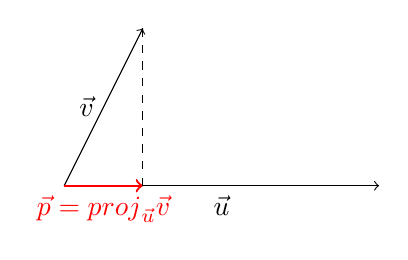
\begin{tikzpicture}
    \draw[->] (0,0)--(4,0) node[pos=0.5,below] {\( \vec{u} \)};
    \draw[->] (0,0)--(1,2) node[pos=0.5,left] {\( \vec{v} \)};
    \draw[->,red,thick] (0,0)--(1,0) node[pos=0.5,below]
      {\( \vec{p} = \text{proj}_{\vec{u}}\vec{v} \)};
    \draw[dashed] (1,2)--(1,0);
  \end{tikzpicture}
\end{center}
\[ \text{proj}_{\vec{u}}\vec{v} =
  (\frac{\vec{u}\cdot\vec{v}}{\vec{u}\cdot\vec{u}})\vec{u} =
  (\frac{\vec{u}\cdot\vec{v}}{\|\vec{u}\|^2})\vec{u} \]

\subsubsection*{Practice Exercise 48}
Given:
\[ \vec{u} = \begin{bmatrix}2 \\ 3\end{bmatrix}
  \vec{v} = \begin{bmatrix}k+1 \\ k-1\end{bmatrix} \]
Find all values of \( k \) such that \( \vec{u} \) and \( \vec{v} \) are
orthogonal.
\begin{align*}
  \vec{u}\cdot\vec{v} &= 0 \\
  2(k+1)+3(k-1) &= 0 \\
  2k+2+3k-3 &= 0 \\
  5k-1 &= 0 \\
  k &= \frac{1}{5}
\end{align*}

\subsubsection*{Practice Exercise 49}
Given:
\[ \vec{u} = \begin{bmatrix}1 \\ -1 \\ 2\end{bmatrix}
  \vec{v} = \begin{bmatrix}k^2 \\ k \\ -3\end{bmatrix} \]
Find all values \( k \) such that \( \vec{u} \) and \( \vec{v} \) are
orthogonal.
\begin{align*}
  \vec{u}\cdot\vec{v} &= 0 \\
  k^2-k+2(-3) &= 0 \\
  k^2-k-6 &= 0 \\
  (k-3)(k+2) &= 0 \\
  k &= 3\ or \\
  k &= 2
\end{align*}

\subsubsection*{Practice Exercise 50}
Describe all vectors \( \vec{v} = \begin{bmatrix}x \\ y\end{bmatrix} \) that
are orthogonal to \( \vec{u} = \begin{bmatrix}3 \\ 1\end{bmatrix} \).
\begin{align*}
  \vec{u}\cdot\vec{v} &= 0 \\
  3x+y &= 0 \\
  y &= -3x
\end{align*}
\( y \) is a line going through the origin with a slope of -3.

\subsubsection*{Practice Exercise 52}
Under what conditions are the following true for vectors \( \vec{u},\vec{v}
\in\R^2\ or\ \R^3 \).
\[ \|\vec{u}+\vec{v}\| = \|\vec{u}\|+\|\vec{v}\| \]
\begin{align*}
  \|\vec{u}+\vec{v}\|^2 &= (\|\vec{u}\|+\|\vec{v}\|)^2 \\
  (\vec{u}+\vec{v})\cdot(\vec{u}+\vec{v}) &= \|\vec{u}\|^2+
    2\|\vec{u}\|\|\vec{v}\|+\|\vec{v}\|^2 \\
  \vec{u}\cdot\vec{u}+2\vec{u}\cdot\vec{v}+\vec{v}\cdot\vec{v} &=
    \|\vec{u}\|^2+2\|\vec{u}\|\|\vec{v}\|+\|\vec{v}\|^2 \\
  \vec{u}\cdot\vec{v} &= \|\vec{u}\|\|\vec{v}\|
\end{align*}
Since:
\[ \cos\theta = \frac{\vec{u}\cdot\vec{v}}{\|\vec{u}\|\|\vec{v}\|} \]
\( \theta \) must be equal to zero since \( \vec{u}\cdot\vec{v} =
\|\vec{u}\|\|\vec{v}\| \). Therefore, this can only be true for \( \vec{u} =
c\vec{v}, c > 0 \).

\subsubsection*{Practice Exercise 55}
Verify the stated property of distances:
\[ d(\vec{u},\vec{v}) = \|\vec{u}-\vec{v}\| \]
\begin{align*}
  d(\vec{u},\vec{v}) &= \|\vec{u}-\vec{v}\| \\
  &= \|(-1)(\vec{v}-\vec{u})\| \\
  &= |-1|\|\vec{v}-\vec{u}\| \\
  &= d(\vec{v},\vec{u})
\end{align*}

\subsubsection*{Practice Exercise 56}
\[ d(\vec{u},\vec{w}) \le d(\vec{u},\vec{v})+d(\vec{v},\vec{w}) \]
\begin{align*}
  d(\vec{u},\vec{w}) &= \|\vec{u}-\vec{w}\| \\
  &= \|(\vec{u}-\vec{v})+(\vec{v}-\vec{w})\| \\
  &\le \|\vec{u}-\vec{w}\|+\|\vec{v}+\vec{w}\| \\
  &= d(\vec{u},\vec{v})+d(\vec{v},\vec{w})
\end{align*}

\subsubsection*{Practice Exercise 58}
Prove:
\[ \vec{u}\cdot c\vec{v} = c(\vec{u}\cdot\vec{v}) \]
\begin{align*}
  \vec{u}\cdot(c\vec{v}) &= (c\vec{v})\cdot\vec{u} \\
  &= c(\vec{v}\cdot\vec{u}) \\
  &= c(\vec{u}\cdot\vec{v})
\end{align*}

\begin{center}
  You can find all my notes at \url{http://omgimanerd.tech/notes}. If you have
  any questions, comments, or concerns, please contact me at
  alvin@omgimanerd.tech
\end{center}

\end{document}
